\chapter{Проектирование и разработка системы}

Разработка плагина производилась на языке Java с использованием REST API функций в качестве точек входа. Для реализации веб-интерфейса использовался HTML5 с Javascript и библиотекой Jquery.

\section{Функциональность}

\subsection{Выбор отчёта}

Для списка отчётов отправляется HTTP GET-запрос на сервер Pentaho. Для получения отчёта пользователю необходимо выбрать его из списка. После выбора отчёта отправляется GET-запрос на получение отчёта. Отчёт предоставляется в формате JSON и содержит массив данных, а также количество строк и столбцов.

В случае удачного подключения, полученные данные отправляются REST-сервису для дальнейшей возможности работать с ними извне, и генерируется таблица. В случае неудачного подключения, пользователю выводится соответствующее сообщение об ошибке. Такими ошибками могут быть:

\begin{enumerate}
	\item Недоступность сервера;
	\item Неудачная попытка загрузки отчёта.
\end{enumerate}

\subsection{Работа с полученными данными}

При получении GET-запроса на свой URL-адрес, REST-сервис обрабатывает его параметры и по ним собирает массив данных, который отправляется в ответе на запрос.

Веб-интерфейс даёт возможность сгенерировать URL для доступа к желаемым элементам по REST-протоколу. Для начала пользователю необходимо выбрать данные при помощи выделения необходимых заголовков таблицы кликом мыши. Для генерации адреса необходимо нажать на кнопку "Generate URL". Также есть возможность вернуться в меню выбора отчёта кнопкой "Back".

\section{Реализация}

Главная часть приложения состоит из работы с параметрами HTTP-запроса и создания массива данных по полученным параметрам.

\subsection{Структура компонентов и описание}

Приложение состоит из 2 классов. Ниже приведена таблица с этими классами и их описанием. В таблице \ref{tab:classes}

\tabulinesep = 1mm
\begin{longtabu} to \textwidth {| X[c,m] | X[c,m] |}
	\firsthline\hline
	Название класса & Описание\\ \hline
	\endfirsthead
	PentahoDataIntegratorService & Описание методов REST сервиса\\ \hline
	DataSelector& Класс-анализатор, выдающий выборку из массива по параметрам запроса\\ \hline
	\caption{Классы и их описание}
	\label{tab:classes}
\end{longtabu}

\subsection{REST-сервис}

В языке Java определена поддержка REST через Java Specification Request (JSR) 311.\cite{jsr} Эта спецификация называется JAX-RS. Для реализации REST-сервиса в данной работе использовалась библиотека Jersey. Jersey предоставляет классы для имплементации веб-сервера в виде сервлета. Конфигурация сервиса находится в отдельном файле - plugin.spring.xml.

Базовый адрес сервиса:

\begin{lstlisting}[
label={listings:base_addr},
caption={"Базовый адрес сервиса"},
style=java]
http://your\_domain:port/display-name/url-pattern/path\_from\_rest\_class
\end{lstlisting}

Сервер анализирует входящий HTTP запрос и выбирает соответствующий ему класс и метод для ответа. Выбор осуществляется на основе аннотаций в классах и методах. Используемые в работе аннотации представлены в таблице \ref{tab:annotations}:

\tabulinesep = 1mm
\begin{longtabu} to \textwidth {| X[c,m] | X[c,m] |}
	 \firsthline\hline
	Аннотация & Описание\\ \hline
	\endfirsthead
	@PATH(your\_path) & Устанавливает путь на конкатенацию адреса домена и адреса метода\\ \hline
	@GET& Метод является HTTP GET запросом\\ \hline
	@Produces(MediaType)& Какой тип данных будет являться ответом на запрос\\ \hline
	@QueryParam& Какие параметры будут внесены в запрос\\ \hline
	\caption{Основные аннотации, используемые в работе}
	\label{tab:annotations}
\end{longtabu}

В классе, представленном в листинге \ref{listings:integr_addr}, метод будет доступен по адресу base/pattern/export. Он будет являться GET запросом и отправлять ответ пользователю.

\begin{lstlisting}[
label={listings:integr_addr},
caption={"GET запрос сервиса"},
style=java]
@Path("@plugin.java.rest.path.root@")
@GET
@Path("/export")
@Produces(MediaType.APPLICATION_JSON)
public Response getSomeData {
	@QueryParam("heads") String headers;
...
}
\end{lstlisting}

Данный класс-ресурс будет доступен по адресу localhost:8080/pentaho/plugin/api/data-integrator/export?heads=chosen\_headers\_of\_the\_table при запросе типа GET, и пользователю будет возвращаться выборка массива по данным заголовкам в виде JSON строки.

\subsection{Графический интерфейс}

При проектировании графического интерфейса уклон был сделан на интуитивность и скорость работы. 

Для реализации использовалась технология HTML и язык Javascript, а также библиотека Jquery. На рисунках \ref{fig:interface1} и \ref{fig:interface2} показано главное окно, которое открывается пользователю при выборе владки плагина и окно сгенерированного отчёта. За дизайн отвечает css код, находящийся в отдельном файле.

\begin{figure}[htbp]
	\centering
	
\includegraphics[width=.82\textwidth]{fig/chapter_4/interface1}
	\caption{Стартовое окно интерфейса плагина}
	\label{fig:interface1}
\end{figure}

Стартовая страница выглядит как селектор с кнопкой подтверждения. 

\begin{figure}[htbp]
	\centering
	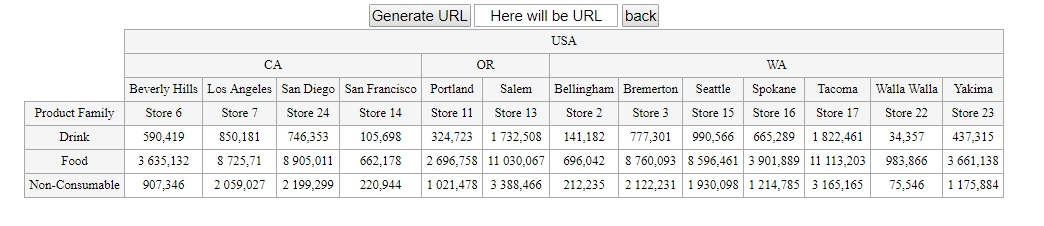
\includegraphics[width=.82\textwidth]{fig/chapter_4/interface2}
	\caption{Пример сгенерированной таблицы}
	\label{fig:interface2}
\end{figure}

На окне работы с отчётом выше таблицы имеются 3 элемента:

\begin{itemize}
	\item Кнопка "Назад" для возвращения обратно на стартовую страницу;
	\item Кнопка "generateURL" для генерации URL по выделенным заголовкам таблицы;
	\item Поле, в которое выводится сгенерированный URL.
\end{itemize}

Реализацию Javascript функций можно найти в приложении 2. В таблице \ref{tab:jsfunc} указаны основные функции.

\tabulinesep = 1mm
\begin{longtabu} to \textwidth {| X[c,m] | X[c,m] |}
	\firsthline\hline
	Функция & Комментарий\\ \hline
	\endfirsthead
	getFiles() & Функция получения списка файлов аналитических отчётов Pentaho BI\\ \hline
	getData() & Функция загрузки данных выбранного отчёта\\ \hline
	createTable() & Функция генерации таблицы по полученным данным\\ \hline
	generateURL() & Функция создания URL на основе выбранных данных\\ \hline
	\caption{Основные функции Javascript-части программы}
	\label{tab:jsfunc}
\end{longtabu}

\section{Итоги}

Было разработано приложение-плагин для Pentaho BI server, в частности, для Pentaho User Console. Данное приложение реализует интеграцию модуля OLAP-анализа платформы Pentaho в CRM-систему посредством предоставления доступа к уже готовым отчётам, хранящимся на сервере Pentaho BI.